
\section{Introduction \DDC}
\label{chap2:intro}
In the past few years, Body Biasing Injection has been getting more and more attention.
Indeed, it is a low-cost method which requires a low bill of material, roughly compsoed of:
\begin{itemize}
    \item A voltage pulse generator
    \item A metallic probe
    \item A target IC
    \item Cables to interconnect equipment
\end{itemize}
The most expensive piece of equipment is definitely the voltage pulse generator.
However, there are low-cost solutions like the NewAE ChipSHOUTER for example, which can easily replace high voltage high precision generator in some use cases.

\subsection{Platform equipment}
\label{chap2:intro:platEquip}
This section is dedicated in presenting the different piece of equipment which allowed us to perform this work.
The hardware platform, as well as the different software used are introduced.


%\begin{figure}[H]
%    \centering
%    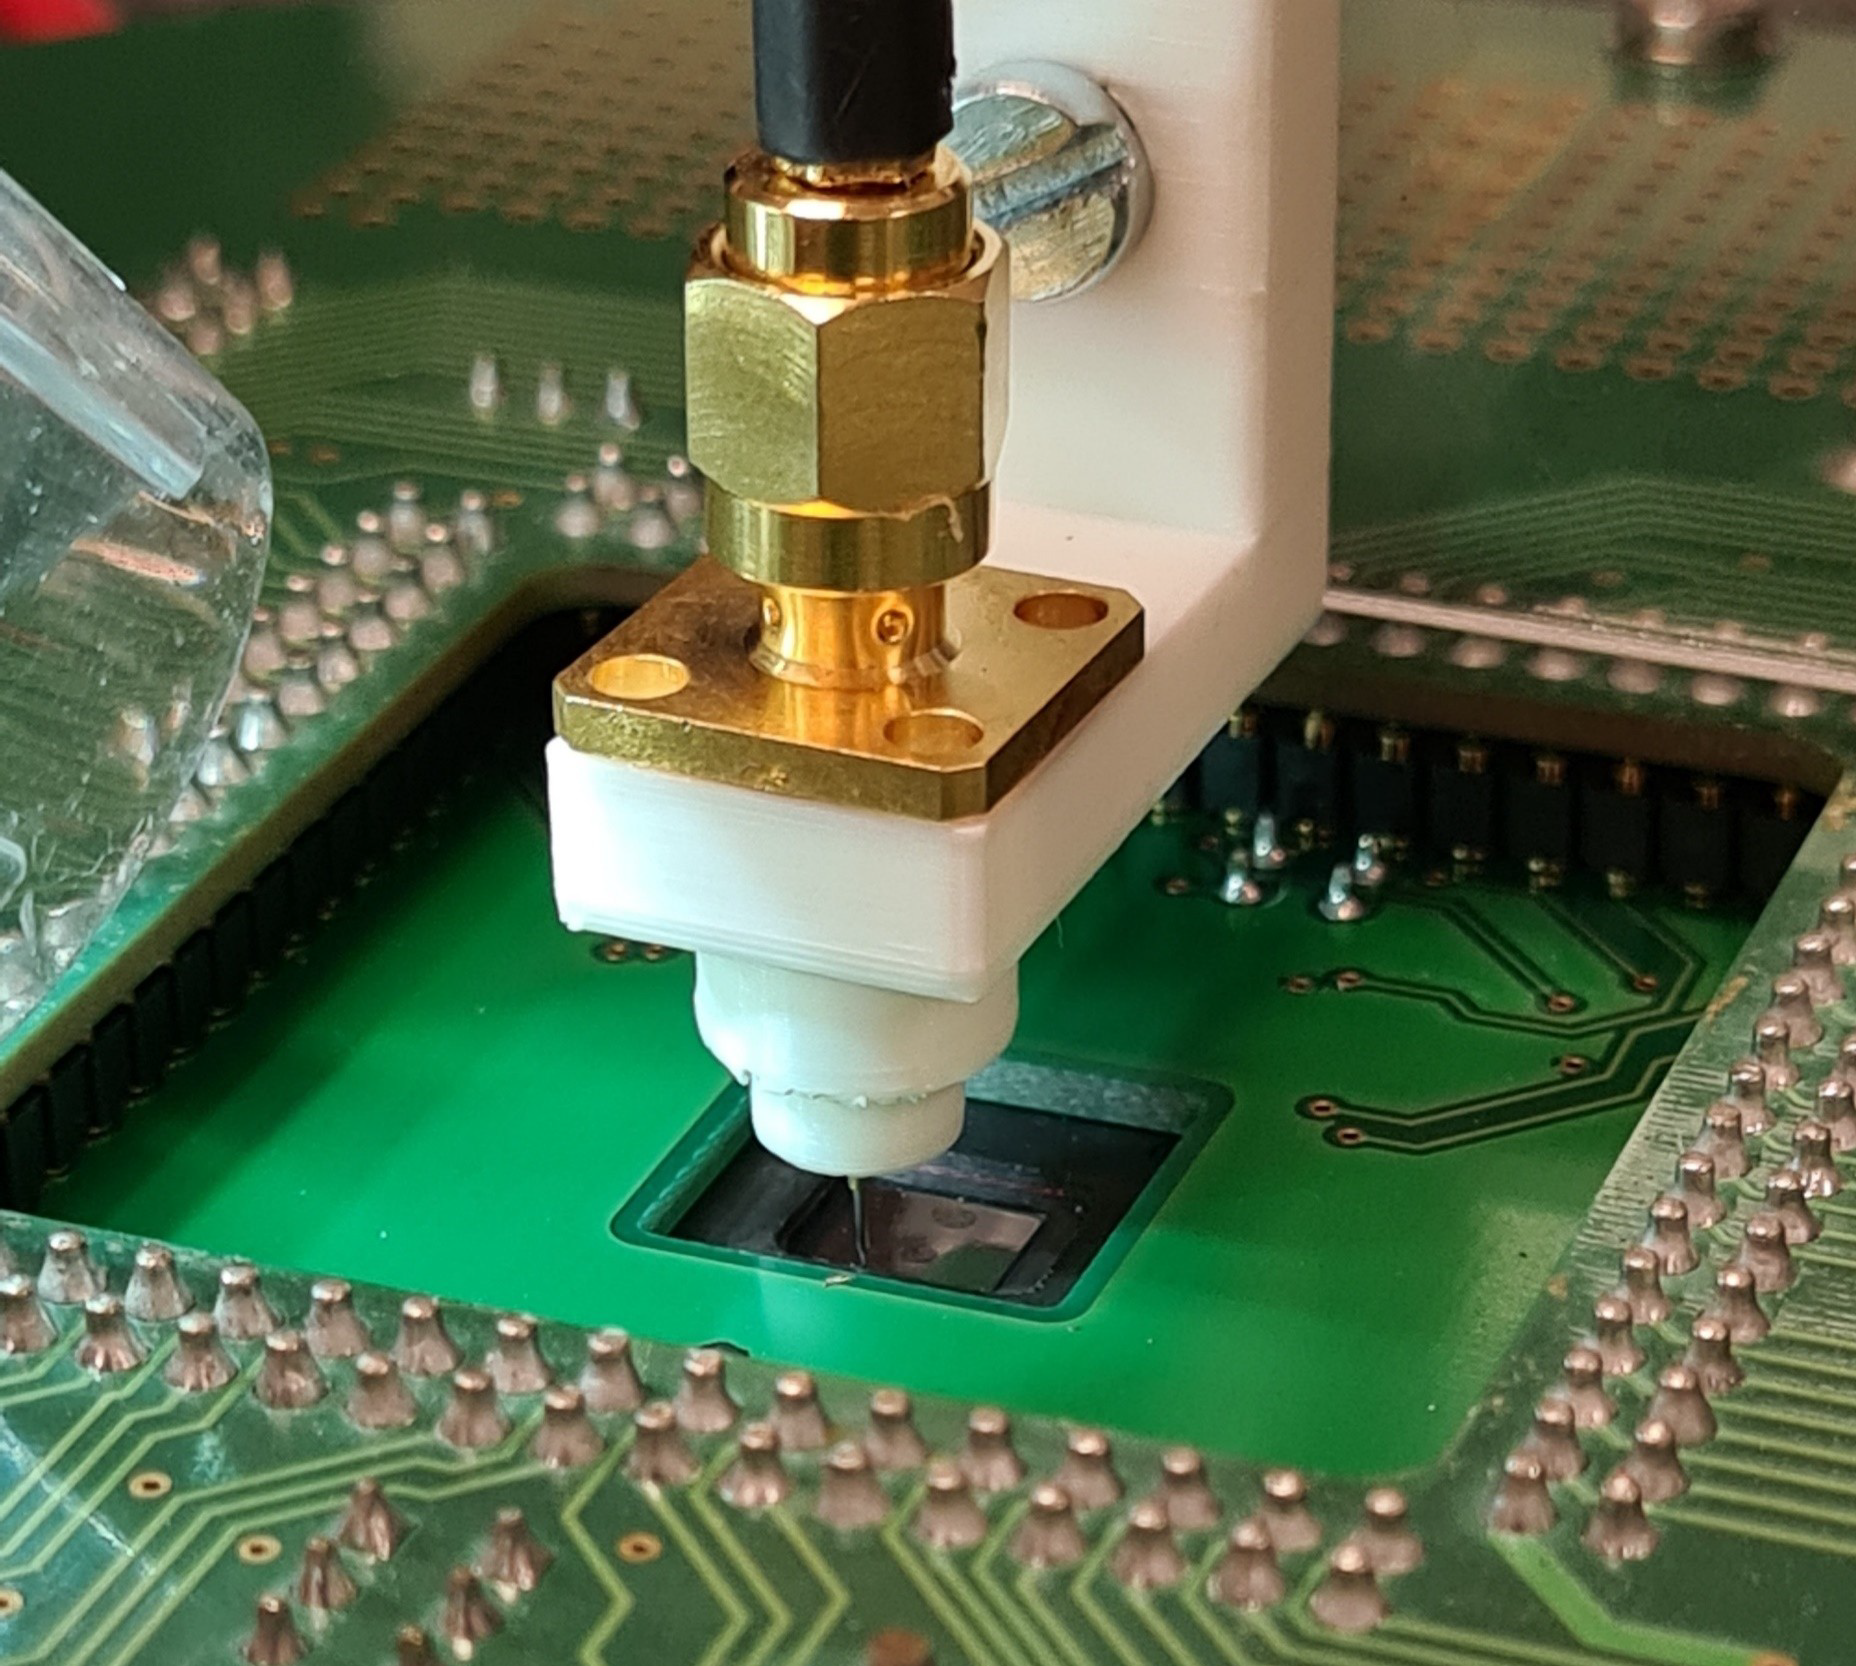
\includegraphics[width=16cm]{2_goodPractices/figures/sondeBBI_loin_raw.png}
%    \caption{BBI metallic probe in mechanical contact with IC target}
%    \label{fig:sondeBBI}
%\end{figure}
%
%\begin{figure}[H]
%    \centering
%    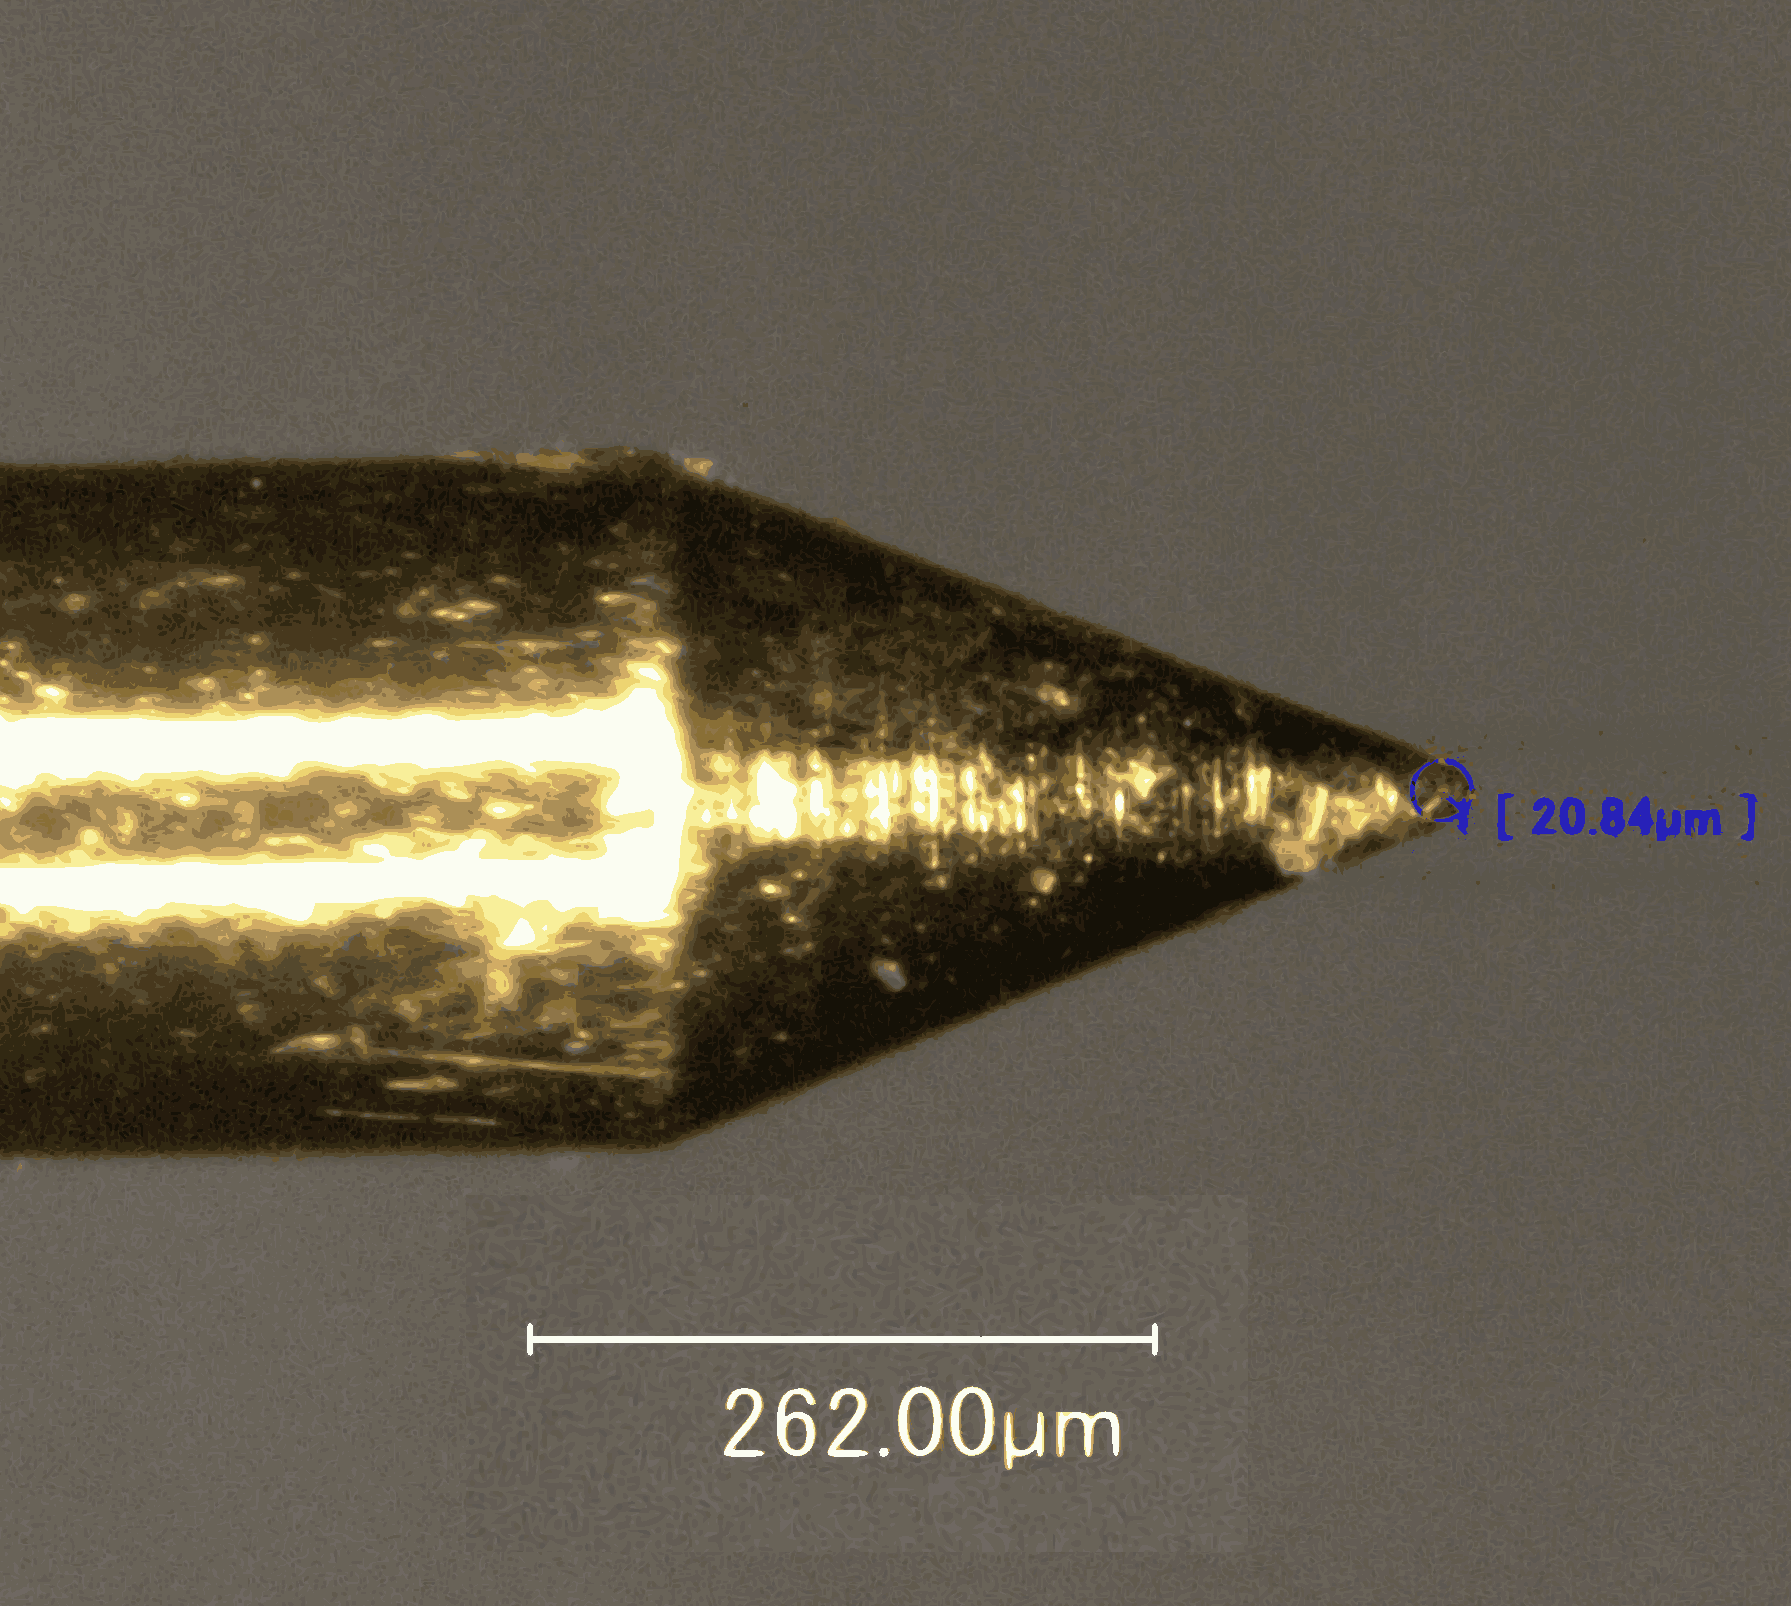
\includegraphics[width=16cm]{2_goodPractices/figures/pointeBBI.pdf}
%    \caption{BBI metallic probe measurement closer look}
%    \label{fig:pointeBBI}
%\end{figure}

\begin{figure}[ht!]
    \centering
    \begin{subfigure}[t]{7.0cm}
        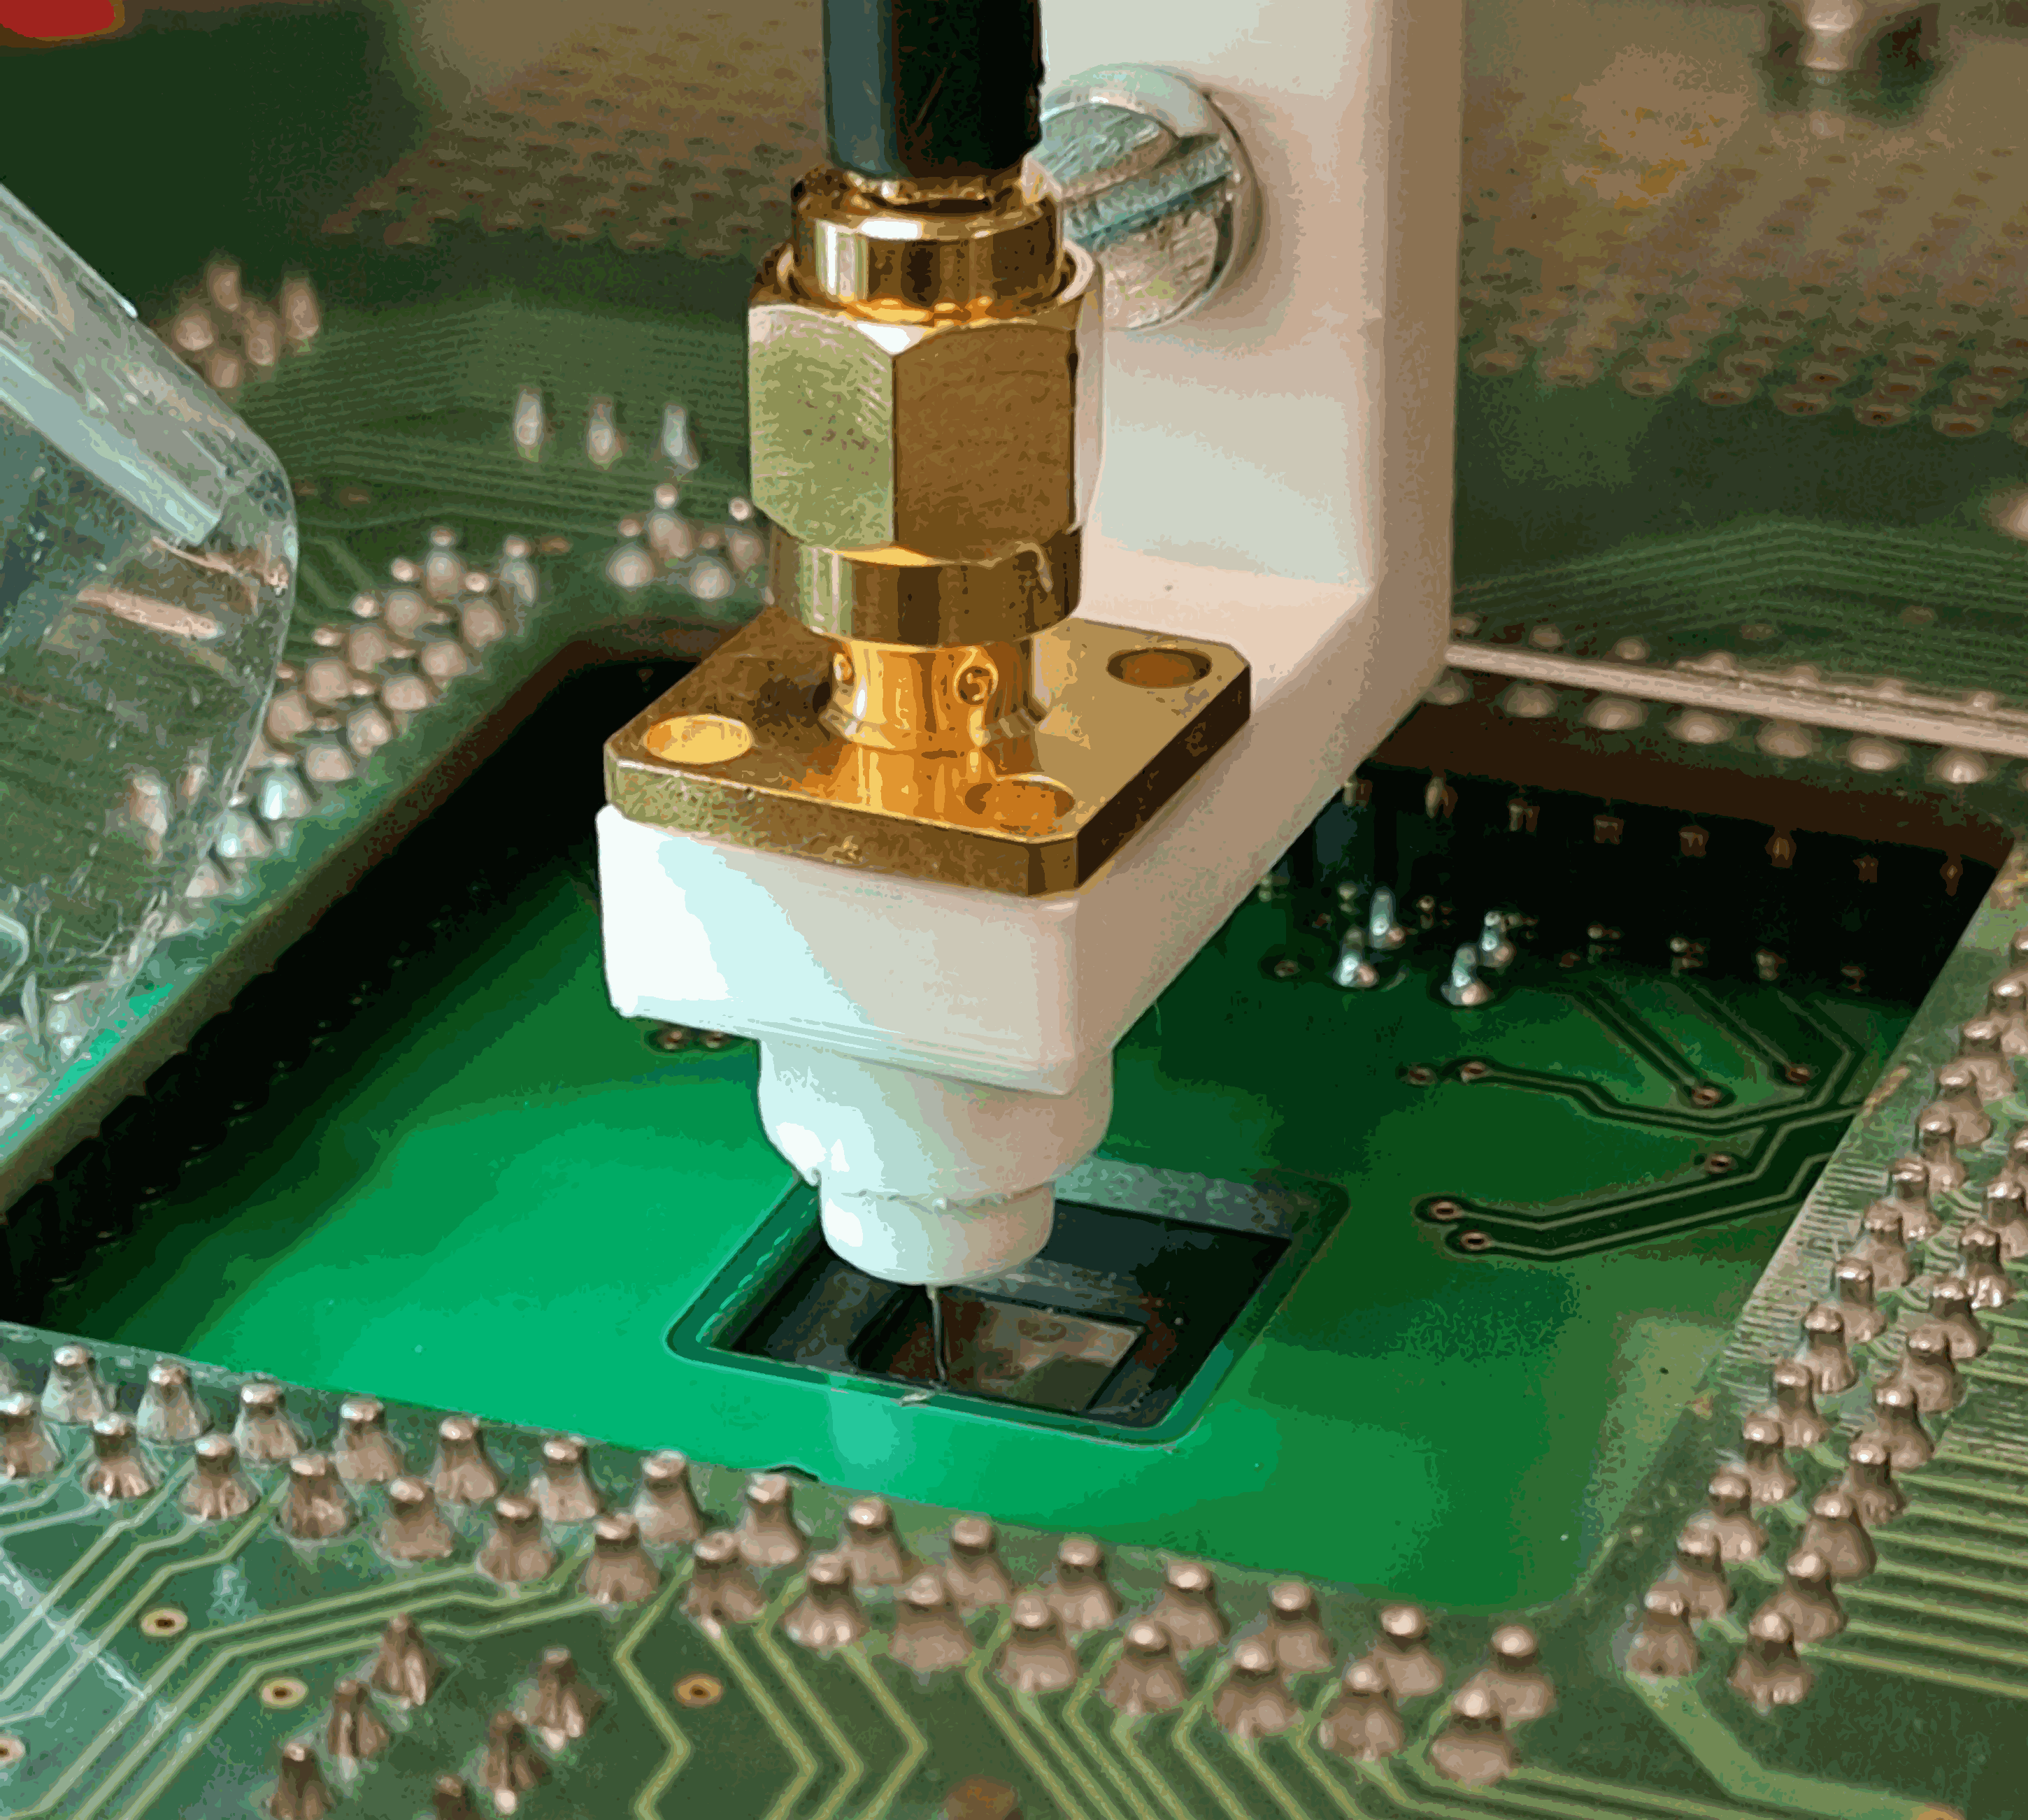
\includegraphics[height=6.8cm]{2_goodPractices/figures/sondeBBI.pdf}
        \caption{BBI metallic probe in mechanical contact with IC target}
        \label{subfig:sondeBBI}
    \end{subfigure}\hfill
    \begin{subfigure}[t]{7.0cm}
        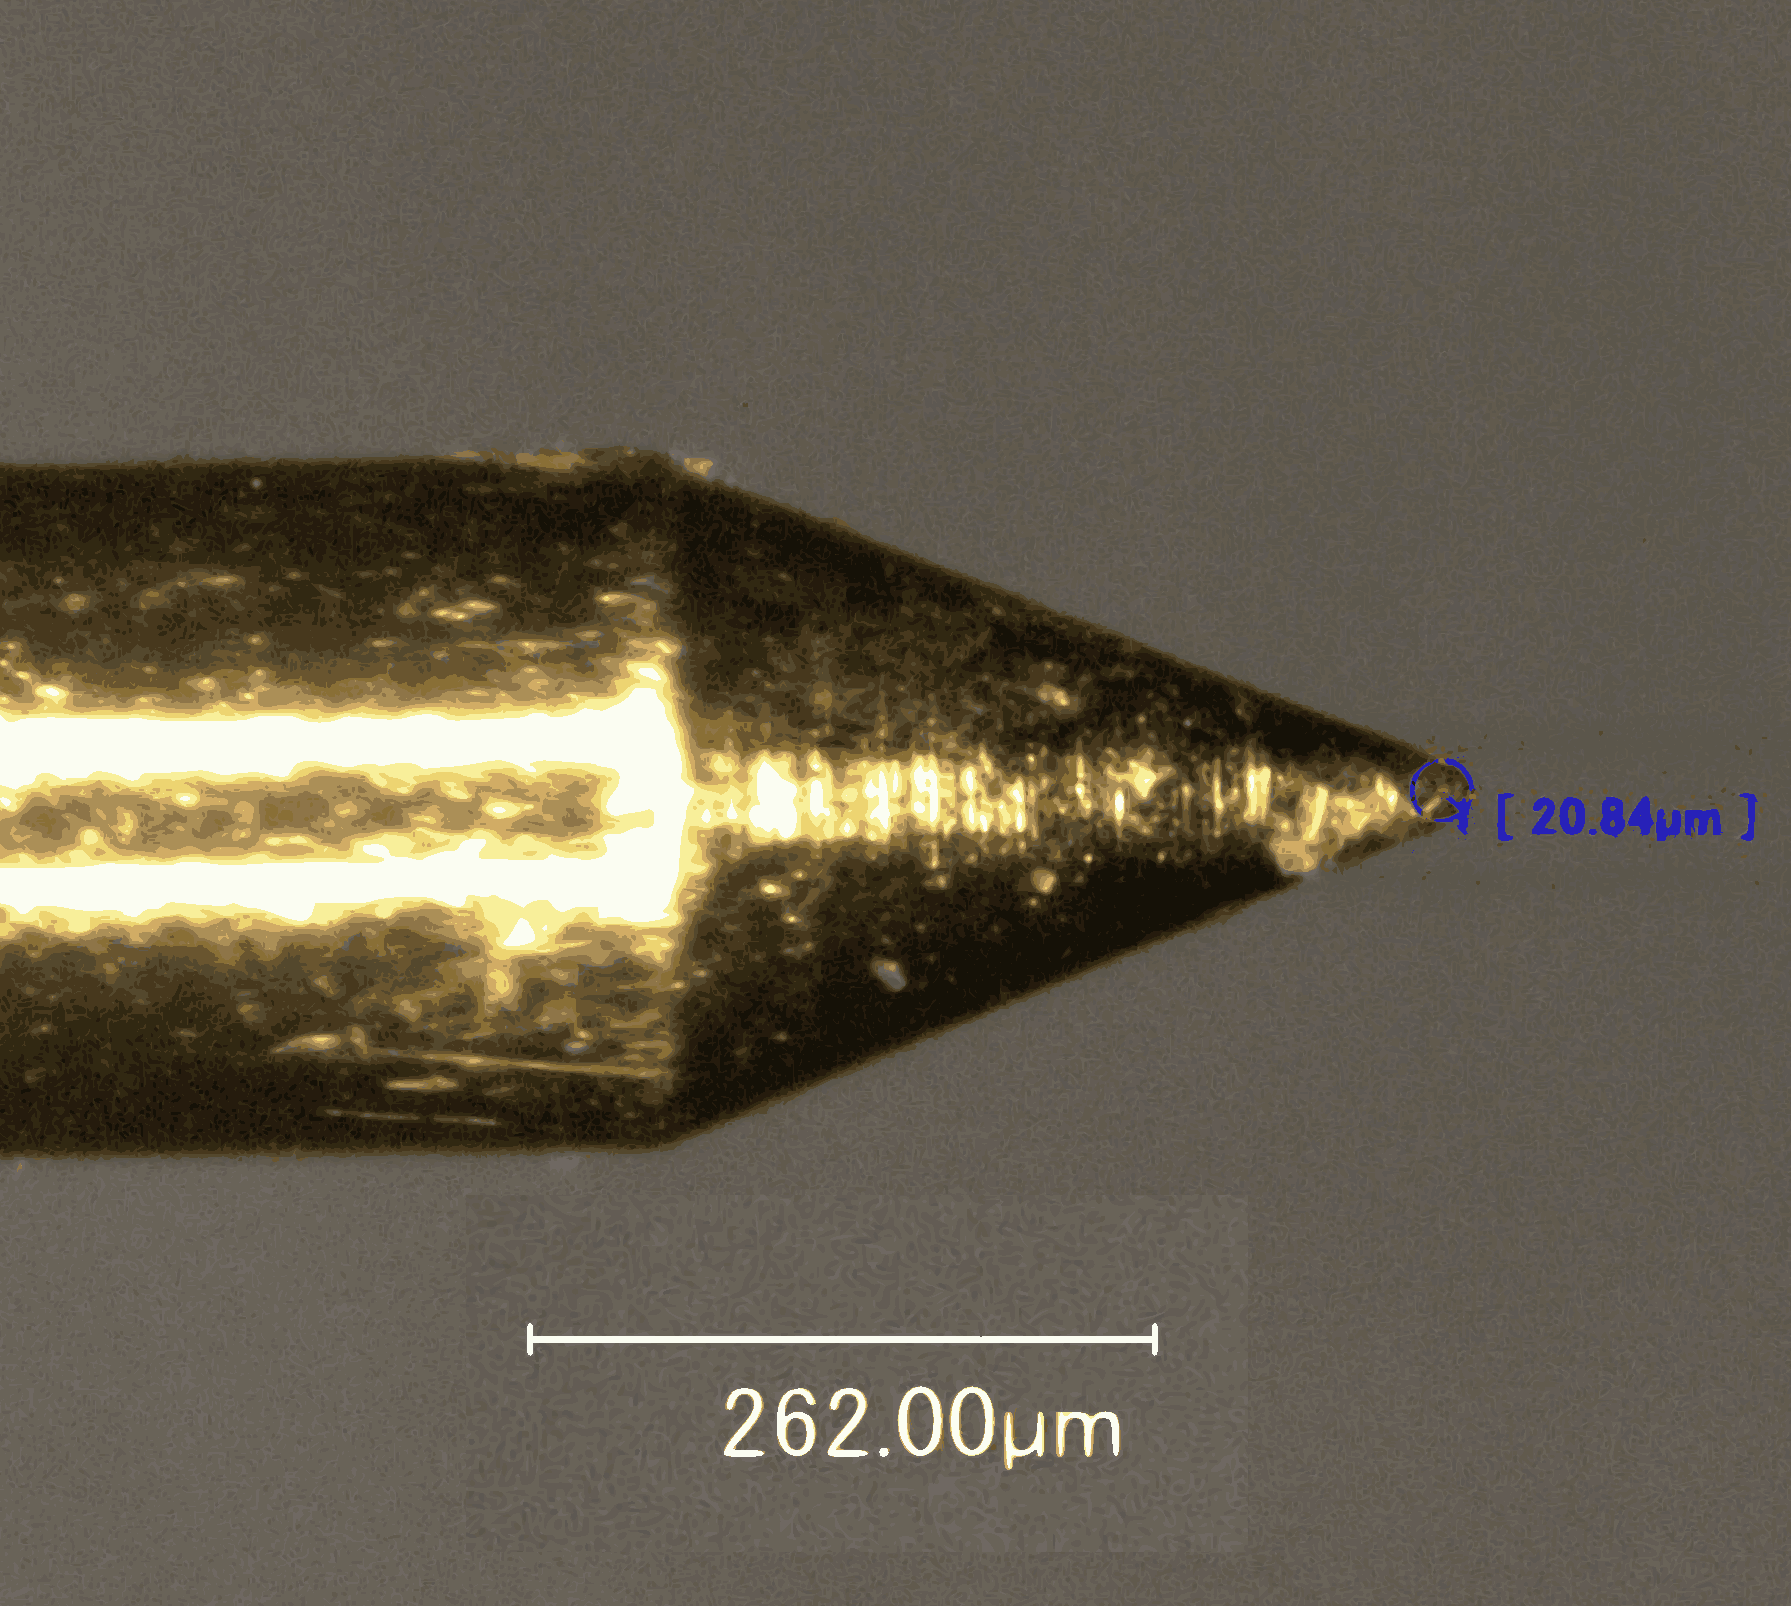
\includegraphics[height=6.8cm]{2_goodPractices/figures/pointeBBI.pdf}
        \caption{BBI metallic probe measurement closer look}
        \label{subfig:pointeBBI}
    \end{subfigure}
    \caption{Dual-well and triple-well inverter silicon sectional view.}
    \label{fig:sondePointeBBI}
\end{figure}
%Nonetheless, during this work, the generator used is the AVTECH AVRK-4-B, which a high speed, precise, voltage pulse generator.
%It allows generating positive or negative pulses up to 750 V of amplitude with a 4 ns rise or fall time, with pulse widths ranging from 6 ns to 20 ns.
%It allowed us to finely tune each setting in order to perform reproducible experiments.
%
%Another very important piece of equipment used for BBI is the probe.
%It simply consists in a metallic tip soldered to an SMA connector.
%However,